\section{Training Details}

\paragraph{High-Quality Fine-Tuning.}
Since the filtered pre-training data still contains a certain proportion of dirty data, such as subtitles, watermarks, and low-bitrate videos, we selected a subset of higher quality video data, accounting for 20\% of the total dataset, for fine-tuning in the final stage. This step effectively removed generated subtitles and watermarks and slightly improved the visual quality. However, we also observed a slight degradation in the model's semantic ability.

\paragraph{Visualizing different rope interpolation methods}
When adapting low-resolution position encoding to high-resolution, we consider two different methods: interpolation and extrapolation. We show the effects of two methods in Figure~\ref{fig:ive}. Interpolation tends to preserve global information more effectively, whereas the extrapolation better retains local details. Given that RoPE is a relative position encoding, We chose the extrapolation to maintain the relative position between pixels. 
\begin{figure}[h]
\begin{center}
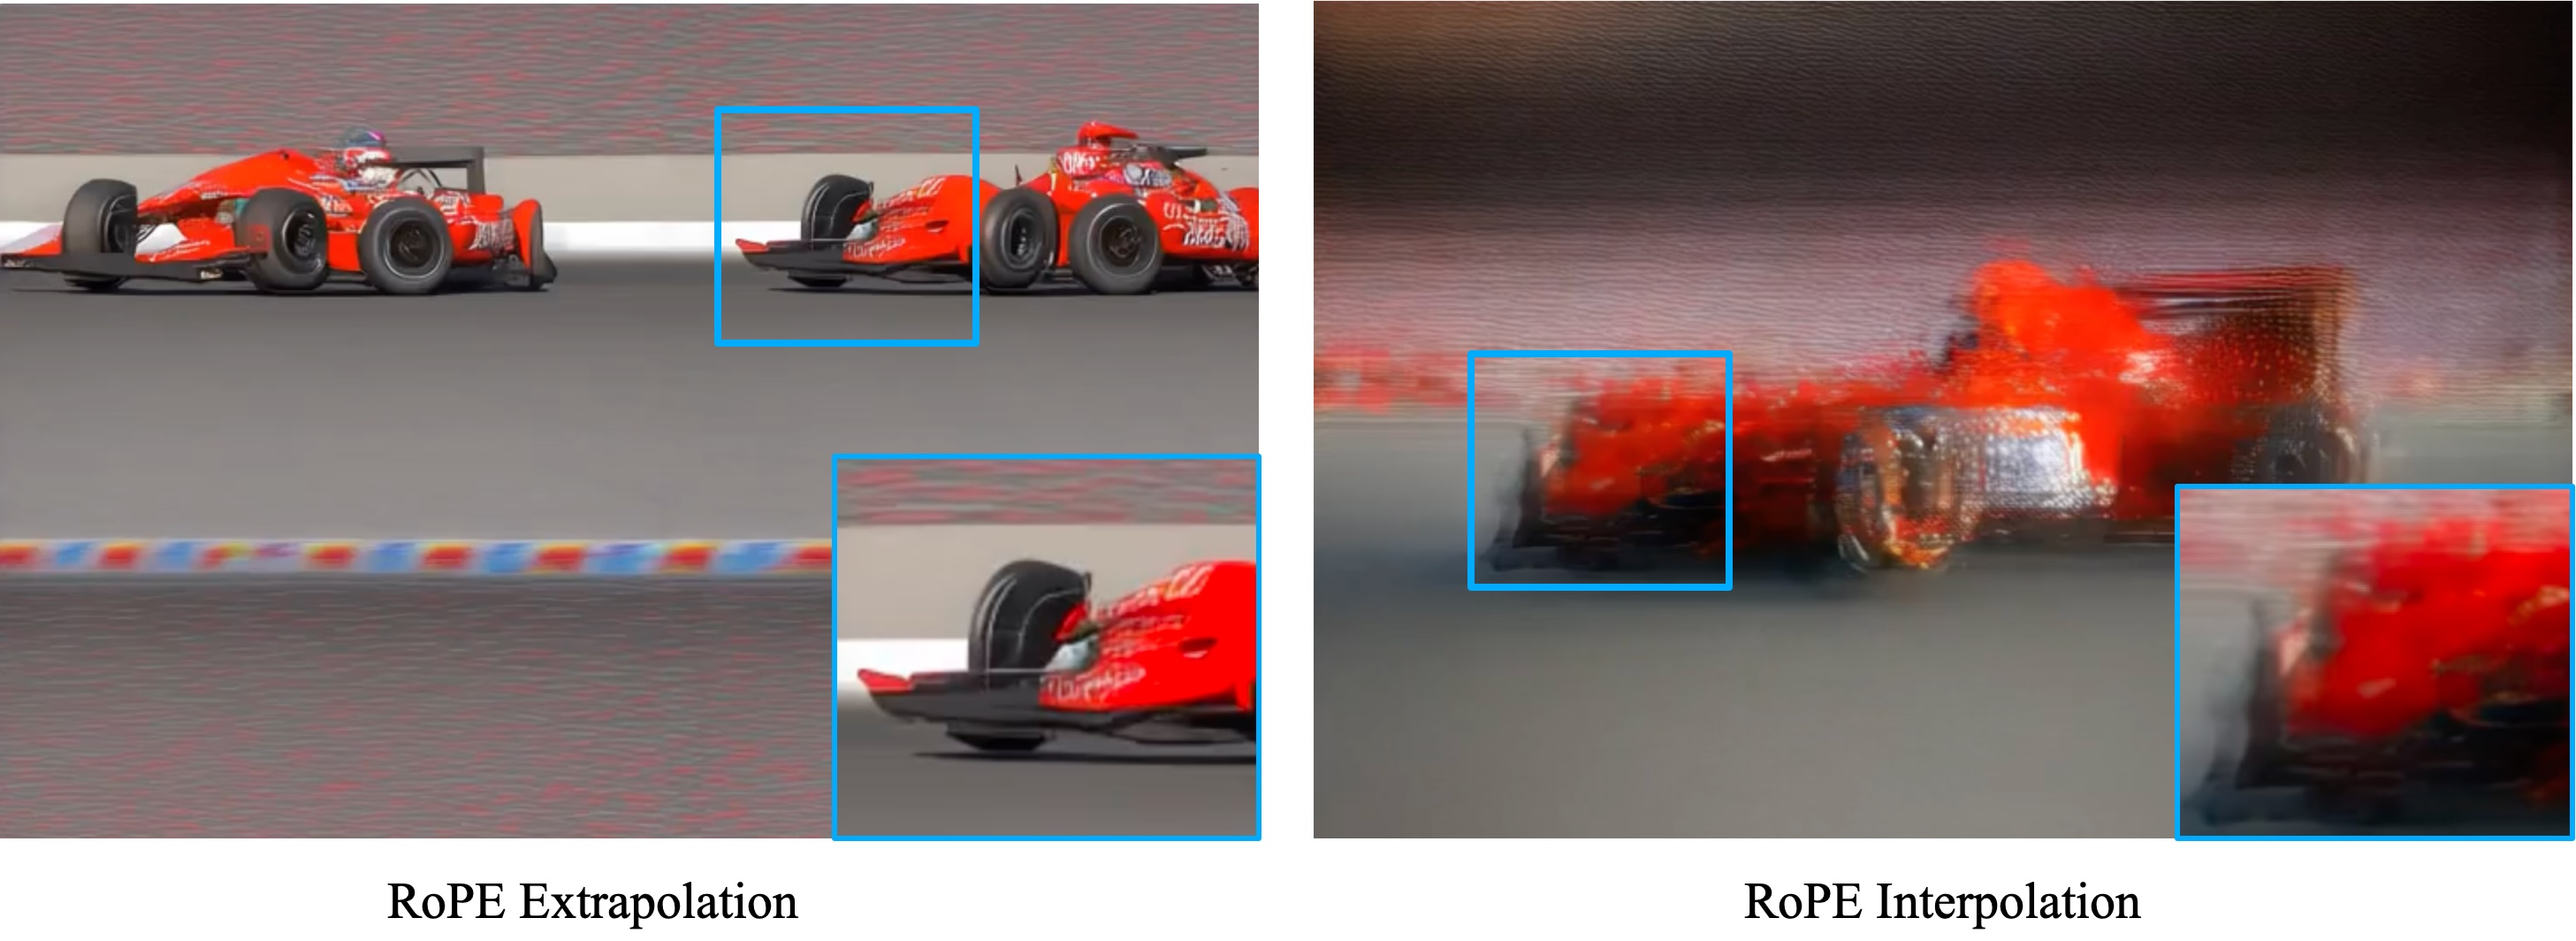
\includegraphics[width=0.7\linewidth]{images/ive.jpg}
\end{center}
\caption{The comparison between the initial generation states of extrapolation and interpolation when increasing the resolution with RoPE. Extrapolation tends to generate multiple small, clear, and repetitive images, while interpolation generates a blurry large image.}
\label{fig:ive}
\end{figure}

\vspace{-2em}
\paragraph{Model \& Training Hyperparameters}
We present the model and training hyperparameters in \cref{tab:hyper2} and \cref{tab:hyper}.

\begin{table}[htbp]
\centering
\small
\begin{tabular}{ccccc}
\toprule
\textbf{Training Stage} & \textbf{stage1} & \textbf{stage2} & \textbf{stage3} & \textbf{stage4 (FT)} \\ 
\midrule
Max Resolution & 256$\times$384 & 480$\times$720 & 768$\times$1360& 768$\times$1360 \\
Max duration & 6s & 6s & 10s & 10s \\
Batch Size & 2000 & 1000 & 250 & 100 \\
Sequence Length & 25k & 75k & 700k & 700k \\
Training Steps & 400k & 220k & 120k & 10k \\

\bottomrule
\end{tabular}
\caption{Hyperparameters of CogvideoX-2b and CogVideo-5b.}
\label{tab:hyper2}
\end{table}

\begin{table}[htbp]
\centering
\small
\vspace{-2em}
\begin{tabular}{ccc}
\toprule
\textbf{Hyperparameter} & \textbf{CogvideoX-2b} & \textbf{CogVideo-5b} \\ 
\midrule
Number of Layers & 30 & 42 \\ 
Attention heads & 32 & 48 \\ 
Hidden Size & 1920 & 3072 \\
Position Encoding & sinusoidal & RoPE \\
Time Embedding Size & \multicolumn{2}{c}{256} \\
Weight Decay & \multicolumn{2}{c}{1e-4} \\
Adam $\epsilon$ & \multicolumn{2}{c}{1e-8} \\
Adam $\beta_1$ & \multicolumn{2}{c}{0.9} \\
Adam $\beta_2$ & \multicolumn{2}{c}{0.95} \\
Learning Rate Decay & \multicolumn{2}{c}{cosine} \\
Gradient Clipping & \multicolumn{2}{c}{1.0} \\
Text Length & \multicolumn{2}{c}{226} \\ 
Max Sequence Length & \multicolumn{2}{c}{82k} \\
Lowest aesthetic-value & \multicolumn{2}{c}{4.5} \\
Training Precision & \multicolumn{2}{c}{BF16} \\
\bottomrule
\end{tabular}
\caption{Hyperparameters of CogvideoX-2b and CogVideo-5b.}
\label{tab:hyper}
\end{table}



% params:
%   time_embed_dim: 512
%   elementwise_affine: True
%   num_frames: 49
%   time_compressed_rate: 4
%   latent_width: 90
%   latent_height: 60
%   num_layers: 30
%   patch_size: 2
%   in_channels: 16
%   out_channels: 16
%   hidden_size: 1920
%   adm_in_channels: 256
%   num_attention_heads: 30

%      target: dit_video_concat.DiffusionTransformer
% params:
%   time_embed_dim: 512
%   elementwise_affine: True
%   num_frames: 49
%   time_compressed_rate: 4
%   latent_width: 90
%   latent_height: 60
%   num_layers: 42
%   patch_size: 2
%   in_channels: 16
%   out_channels: 16
%   hidden_size: 3072
%   adm_in_channels: 256
%   num_attention_heads: 48